% 原书 p.120–p.125（PDF p.128–p.133）
% 第 5 章 5.3 节：同调刚性（Homological Rigidity）
% 说明：本章 \chapter 标题由 ch05a 译者写出；p.120 页首两段（5.2 节结尾，含 p128 页标记）
%       亦由 ch05a 负责。本文件从 \section{同调刚性} 开始，不重复该两段。

\section{同调刚性（Homological Rigidity）}
% >>> p128

\begin{keytakeaways}
\begin{itemize}
  \item 几何图像：辛几何中的刚性（rigidity）表现为「临界点、不动点、相交点、周期轨道、Reeb 弦」
        数量的下界；这些下界只由底流形的拓扑（Betti 数）决定，与度量、扰动无关。
  \item 数学工具：有限维 Morse 同调给出原型 $\#\Crit(F)\geqslant\sum_i b_i$；辛情形用
        Hamilton Floer 同调与 Lagrangian Floer 同调替代；切触情形则把闭轨换成 Reeb 弦。
  \item 本节结论：Arnold 猜想（猜想 5.3.1、5.3.2）、Arnold 弦猜想（猜想 5.3.3、5.3.4）、
        Conley 猜想（猜想 5.3.5）、Hofer--Zehnder 猜想（猜想 5.3.6）以及切触版本的
        猜想 5.3.7；例 5.3.4--例 5.3.5 还揭示出动力学中的「二分性」。
  \item 阅读要点：各猜想的下界都形如 $\sum_i b_i$（或其一半），核对时先确认系数域 $\mathbf{k}$
        与 Betti 数的取值范围；「刚性」与「二分化」是同一现象的两个侧面。
\end{itemize}
\end{keytakeaways}

从 Morse 同调出发，我们已经看到 Morse 函数具有某种刚性。例如，临界点的个数满足
\[
  \#\Crit(F)\geqslant\sum_i b_i(X;\mathbf{k}).
\]
在辛几何中同样会出现刚性现象。本节将列举辛几何中一批著名猜想——刚性在其中以不同的形态登场。
% [Tutor Note: 原文疑误——此处 $X$ 在上下文中并无定义，应为底流形 $M$，即应作
%  $\#\Crit(F)\geqslant\sum_i b_i(M;\mathbf{k})$。另请核对：这正是不带重数的「弱 Morse 不等式」
%  （weak Morse inequality），它等价于 Morse 同调复形的存在性，即 $b_i\le c_i$（$c_i$ 为指标
%  $i$ 的临界点个数）对每个 $i$ 成立再求和；它不是从 Morse 函数的梯度流直接数出来的，
% 而需要 Morse 同调这条链。经典参考：Milnor, *Morse Theory*, Princeton Univ. Press, 1963,
% 第 5 节。详见 qsg/notes/review_ch05b.md。]

\begin{wconj}{5.3.1}（Arnold 猜想——哈密顿版本, Arnold conjecture-Hamiltonian version）
  对任意紧辛流形 $(M,\omega)$ 与非退化的哈密顿函数 $H\colon[0,1]\times M\to\R$，有
  \begin{equation*}
    \#\{\text{时间-}1\text{ 映射 }\varphi_H^1\text{ 的不动点}\}
      \geqslant\sum_i b_i(M;\mathbf{k}),
  \end{equation*}
  其中 $b_i(M;\mathbf{k})$ 表示 $M$ 的第 $i$ 个 Betti 数（系数域为 $\mathbf{k}$）。
\end{wconj}
% [Tutor Note: 易错预警（三处）——(1) 原文写作「fix points」，系 fixed points 的漏字，
%  译文按「不动点」处理；(2) 下界对每个时间-1 映射 $\varphi_H^1$ 计数，哈密顿函数 $H$ 的
%  「非退化」是指 $\varphi_H^1$ 的每个不动点 $x$ 都满足 $\det(\mathbf{1}-(\varphi_H^1)_{*x})\ne0$
%  （定义 5.4.1），此时不动点集离散，$\#$ 才有意义，否则须按 Conley--Zehnder 的约定计重数；
%  (3) 这里的 $\varphi_H^1$ 是哈密顿流的时间-1 映射，而非任意辛同胚，两类映射的刚性行为不同
%  （对比例 5.3.2）。]

对哈密顿函数的非退化性，见定义 5.4.1。

猜想 5.3.1 已在许多情形得到证明，包括所有闭定向曲面、复射影空间等等。这些证明的难度依辛流形的
复杂程度而不同。主要工具是哈密顿 Floer 同调理论，其基本版本将在 5.4 节详细展开。这一理论由
Arnold 在 20 世纪 60 年代提出（见 [13]、[15] 的附录 9、[16] 的 Problem 1972-33），其完整版本
在 [82, 121, 148, 89] 中建立起来，并在 [175, 7] 中有更新。
% [Tutor Note: 含糊点拨——原文「the full version this theory is built up in …」漏了 of，
%  应按「该理论的完整版本见 […]」理解。此处「完整版本」指去掉对 $\pi_2(M)$ 与第一 Chern 类
%  的限制（即 (5.16) 的辛非球面条件），用 Novikov 环与虚拟模技术处理一般紧辛流形；
%  5.4 节只做辛非球面的情形。对照阅读时可留意 5.4 节定理 5.4.1 与猜想 5.3.1 的条件差异。]

\begin{wexam}{5.3.1}
  对 $\R^3$ 中的标准 2-球面 $(S^2,\omega_{\mathrm{area}})$，由猜想 5.3.1（在这一情形它其实是定理），
  任何非退化哈密顿函数 $H\colon[0,1]\times S^1\to\R$ 的时间-1 映射至少有两个不动点。这个数 $2$
  是最优的，因为沿 $z$ 轴的旋转即可达到（见图 5.13）。\hfill$//$
\end{wexam}
% [Tutor Note: 原文疑误——上式中 $H$ 的定义域写成 $[0,1]\times S^1$，但本例题的底流形是
%  $S^2$，应为 $[0,1]\times S^2\to\R$。译文保留原文写法，详见 qsg/notes/review_ch05b.md。]

\begin{wexam}{5.3.2}
  （参看练习 1.7.5）在标准 2-环面 $(\T^2,\omega_{\mathrm{area}})$ 上，沿 $\T^2$ 的某个 $S^1$-因子
  作足够小的、非周期的旋转，\textbf{不能}实现为任何哈密顿流的时间-1 映射（因为它的时间-1 映射
  将没有不动点），这与猜想 5.3.1 矛盾（这一情形它同样是定理）。\hfill$//$
\end{wexam}
% [Tutor Note: 易错预警——此例的关键在于「辛同胚」与「哈密顿微分同胚」的差别：$\T^2$ 上沿
%  $S^1$-因子的平移是辛同胚（保持 $\dd x\wedge\dd y$），其生成函数 $H=ay-bx$ 在 $\T^2$ 上不是
%  单值函数，故该平移落在 $\Symp(\T^2)\setminus\Ham(\T^2)$ 中（其通量非零）。因此它没有不动点
%  并不违反 Arnold 猜想；只有当映射属于 $\Ham$ 时下界才成立。原文的括号说明正是这个意思。]

在给出任何证明之前，先看一个支持猜想 5.3.1 的证据。给定一个与时间无关的 Morse 函数
$F\colon M\to\R$，把它视为一个哈密顿函数。
% >>> p129
\begin{figure}[htbp]
  \centering
  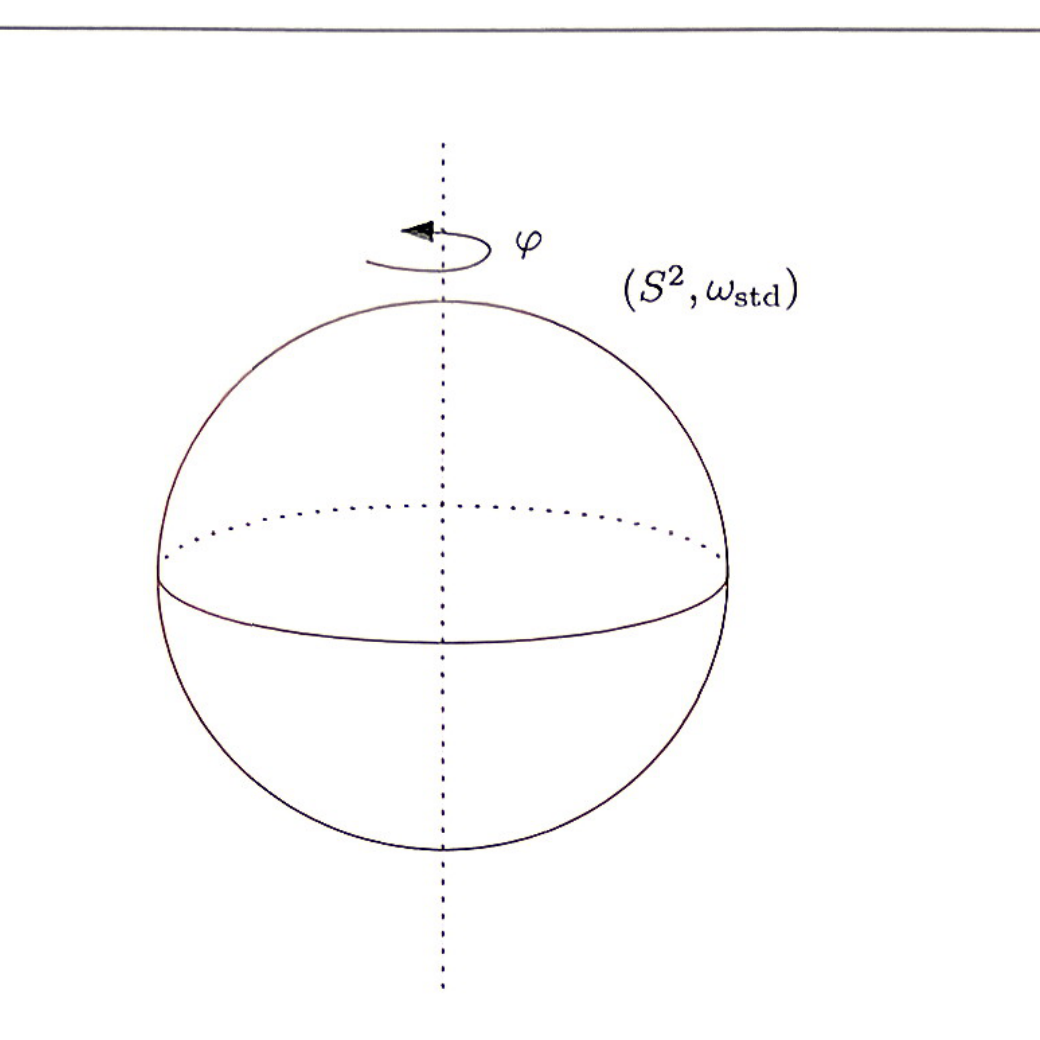
\includegraphics[width=0.42\linewidth]{figures/fig_p129_1.png}
  \caption*{图 5.13\quad $S^2$ 沿 $z$ 轴的旋转（原书 p.121, Figure 5.13）}
\end{figure}

那么任何 $p\in\Crit(F)$ 都由 $F$ 的哈密顿向量场 $X_F$ 的定义关系
$-\dd F=\omega(X_F,\cdot)$ 满足 $X_F(p)=0$。特别地，$p$ 是一条常值的哈密顿轨道，从而是时间-1
映射 $\varphi_F^1$ 的不动点。于是
\[
  \#\{\varphi_F^1\text{ 的不动点}\}\geqslant\#\Crit(F)\geqslant\sum_i b_i(M;\mathbf{k}),
\]
其中最后一个不等式来自 5.1 节的 Morse 理论。因此，在这一特殊情形我们容易地验证了猜想 5.3.1。
% [Tutor Note: 易错预警——注意 $\varphi_F^1$ 的下标是函数 $F$ 而不是 $H$：与时间无关的 $F$ 生成
%  哈密顿流 $\varphi_F^t$，而 $\Crit(F)$ 就是该流的不动点集（因为 $X_F(p)=0$ 当且仅当 $p$ 是
%  $\varphi_F^t$ 的不动点）。符号约定也请统一：本书采用 $\iota_{X_F}\omega=-\dd F$（等价地
%  $\omega(X_F,\cdot)=-\dd F$），与不少教材采用的 $\iota_{X_H}\omega=\dd H$ 相差一个负号；
%  后文 (5.20)、(5.21) 的梯度流方程都依赖于这一约定，换约定时须整体改号。]

\begin{wexer}{5.3.1}
  证明：对任何与恒同映射 $C^1$-接近的哈密顿流的时间-1 映射，猜想 5.3.1 都成立
  （提示：例 4.3.1）。
\end{wexer}

稍后在 5.4 节中，我们将证明猜想 5.3.1 对一族特殊的辛流形成立（它们满足条件 (5.16)）。
这一条件使我们能建立 Morse 理论的一个无穷维版本，即所谓哈密顿 Floer 同调群。于是猜想 5.3.1
成为该同调理论某条不变性质的直接推论（见定理 5.4.1）。

下面是猜想 5.3.1 的一个相对版本。

\begin{wconj}{5.3.2}（Arnold 猜想——拉格朗日版本, Arnold conjecture-Lagrangian version）
  设 $(M,\omega)$ 是闭辛流形，$L\subset(M,\omega)$ 是紧拉格朗日子流形。给定哈密顿微分同胚
  $\varphi\in\Ham(M,\omega)$，若 $L$ 与 $\varphi(L)$ 横截相交，则
  \begin{equation*}
    \#(\varphi(L)\cap L)\geqslant\sum_i b_i(L;\mathbf{k}),
  \end{equation*}
  其中 $b_i(L;\mathbf{k})$ 表示拉格朗日子流形 $L$ 的第 $i$ 个 Betti 数（基域为 $\mathbf{k}$）。
\end{wconj}
% [Tutor Note: 术语依据——本书把「横截相交」统一作 transverse intersection；此处 $\#$ 是对
%  交点计数，横截性保证交点离散（若 $L$ 闭紧则交点有限）。另请注意：构造 Lagrangian Floer
%  同调以证明本猜想时，通常还需对 $L$ 附加假设（例如 $L$ 可定向且具有相对 $\mathrm{Spin}$
%  结构、$[\omega]$ 与 Maslov 类满足单调性或半正性），这些假设在原文此处被省略；Floer 的原始
%  工作与 Fukaya--Oh--Ohta--Ono 的专著 [88] 中均有明确陈述。]

% >>> p130
观察到猜想 5.3.2 蕴含猜想 5.3.1。事实上，对任意哈密顿微分同胚 $\varphi=\varphi_H^1$，回忆其图像
$\mathrm{graph}(\varphi)\subset(M\times M,\omega_{\mathrm{twist}}=\pi_1^*\omega-\pi_2^*\omega)$
是拉格朗日子流形（见例 1.6.2）。$H$ 的非退化性条件蕴涵 $\mathrm{graph}(\varphi)$ 与 $M\times M$
的对角线 $\Delta$ 横截相交（见注 5.4.3）。此外，$\mathrm{graph}(\varphi)$ 可看作 $\Delta$ 在
哈密顿微分同胚 $1\times\varphi\in\Ham(M\times M,\omega_{\mathrm{twist}})$ 下的像。于是
猜想 5.3.2 说的是
\[
  \#(\mathrm{graph}(\varphi)\cap\Delta)\geqslant\sum_i b_i(\Delta;\mathbf{k})
    =\sum_i b_i(M;\mathbf{k}).
\]
同时，按定义，$\mathrm{graph}(\varphi)\cap\Delta$ 恰好由 $\varphi$ 的那些不动点组成。因此
$\#(\mathrm{graph}(\varphi)\cap\Delta)=\#\mathrm{Fix}(\varphi)$。这就证明了猜想 5.3.1。
% [Tutor Note: 易错预警——请核对两处符号约定：(1) $\omega_{\mathrm{twist}}=\pi_1^*\omega-\pi_2^*\omega$
%  中两根投影的次序决定了「图像」与「对角线」谁与谁横截，若把 $\omega_{\mathrm{twist}}$ 写成
%  $\pi_2^*\omega-\pi_1^*\omega$，则 $1\times\varphi$ 在 $\omega_{\mathrm{twist}}$ 下仍是哈密顿的，
%  结论不变，但中间各式的正负号会反转；(2) $\mathrm{graph}(\varphi)$ 与 $\Delta$ 横截当且仅当
%  $1$ 不是 $(\varphi_H^1)_{*x}$ 的特征值，即定义 5.4.1 的非退化条件。$\Delta$ 与 $M$ 同胚，
%  故 $b_i(\Delta;\mathbf{k})=b_i(M;\mathbf{k})$，这一步用到了 $M$ 的定向与系数域 $\mathbf{k}$。]

\begin{wexam}{5.3.3}
  在标准 2-球面 $(S^2,\omega_{\mathrm{area}})$ 上，标准赤道 $L$ 是拉格朗日子流形。于是猜想 5.3.2
  蕴涵：对任意 $\varphi\in\Ham(S^2,\omega_{\mathrm{area}})$，有
  \[
    \#(\varphi(L)\cap L)\geqslant\sum_i b_i(L;\mathbf{k})=2.
  \]
  特别地，赤道 $L$ 不能从自身「挪开」（displace），意思是：对任意
  $\varphi\in\Ham(S^2,\omega_{\mathrm{area}})$，总有 $\varphi(L)\cap L\ne\varnothing$（见图 5.14）。
  与此形成鲜明对比的是，若取一个足够小的圆 $L'\subset S^2$（它同样是拉格朗日子流形），则容易
  用某个 $\varphi\in\Ham(S^2,\omega_{\mathrm{area}})$（例如一个旋转或一个反射）把它挪开。这表明：
  小圆与赤道（或更一般地，任何无自交、把 $(S^2,\omega_{\mathrm{area}})$ 分成两个等面积部分的闭曲线）
  尽管都是拉格朗日子流形，却因某种更深刻的辛几何原因而不是「同一类」对象。\hfill$//$
\end{wexam}
% [Tutor Note: 含糊点拨——「不能挪开」即非位移性（non-displaceability）。原文用「equal areas」
%  刻画赤道，是因为 $S^2$ 上的闭曲线若把面积均分，则它是哈密顿同痕意义下「可分」的，
%  这类曲线正是拉格朗日圆；而小圆虽然也是拉格朗日圆，却可以整体挪开（其围成的两块面积不等）。
%  严格的判别要用 Lagrangian Floer 同调或 Hofer 几何；可参看 McDuff--Salamon,
%  *J-holomorphic Curves and Symplectic Topology*, AMS, 2004, 第 9 章。]

\begin{figure}[htbp]
  \centering
  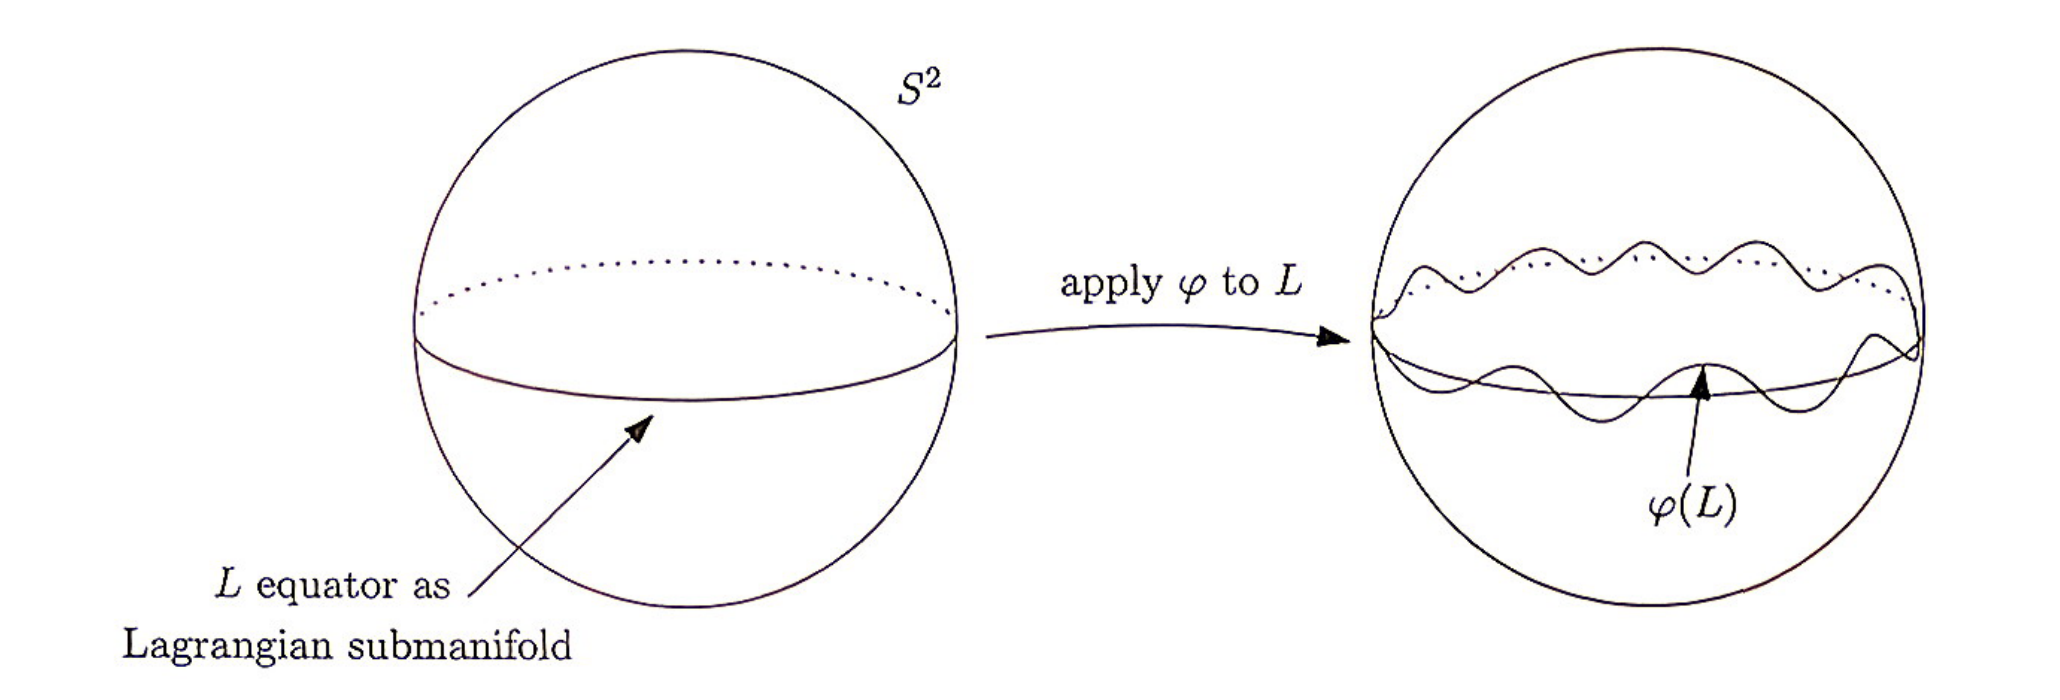
\includegraphics[width=0.86\linewidth]{figures/fig_p130_1.png}
  \caption*{图 5.14\quad $S^2$ 上赤道 $L$ 的非位移性（原书 p.122, Figure 5.14）}
\end{figure}

\begin{wrem}{5.3.1}
  研究子集 $A\subset(M,\omega)$ 的（非）位移性是辛几何中的核心问题之一。如今这一问题已得到
  系统的研究（例如见 [79]）。
\end{wrem}

% >>> p131
与猜想 5.3.1 类似，猜想 5.3.2 也已在许多情形得到证明。支撑它的机器称为\textbf{拉格朗日
Floer 同调理论}（Lagrangian Floer homology theory），已由 Fukaya--Oh--Ohta--Ono 在 [88] 中
完整发展起来。

回忆任何切触流形自身都带有一种（哈密顿型）动力学——基于 Reeb 向量场的 Reeb 动力学（见例 3.5.3）。
下面这个与 Reeb 动力学有关的猜想，是猜想 5.3.2 在切触几何中的对应物。

\begin{wconj}{5.3.3}
  设 $(M,\xi=\ker\alpha)$ 是带固定切触 1-形式 $\alpha$ 的切触流形，$L\subset(M,\xi)$ 是紧
  勒让德子流形。则
  \begin{equation}\tag{5.15}
    \#\{L\text{ 的 Reeb 弦}\}\geqslant\frac12\sum_i b_i(L;\mathbf{k}).
  \end{equation}
\end{wconj}
% [Tutor Note: 术语依据——原文「Reeb chord of L」译作「Reeb 弦」；它指 Reeb 向量场 $R_\alpha$
%  的一条流线，起点与终点都落在 $L$ 上（起点与终点可以重合）。注意 (5.15) 右端带因子 $1/2$：
%  一条 Reeb 弦按两个端点各计一次，故与「弦的条数」相差常数；核对文献时务必先确认其计数约定
%  （有的作者计 $\#$chords，有的计 $\#$Reeb orbits）。]

这里，Reeb 弦指 Reeb 向量场 $R_\alpha$ 的一条流线，它从 $L$ 上出发，最终也落在 $L$ 上
（起点与终点可能重合）。

在切触流形 $(M,\xi=\ker\alpha)$ 与勒让德子流形 $L$ 都满足一定条件时，猜想 5.3.3 已在若干情形
得到证实。见 [50, 185, 65, 72, 71, 147, 191]。

当猜想 5.3.3 中的紧勒让德子流形 $L$ 是可定向子流形时，(5.15) 的右端至少为 $1$。于是该猜想特别地
蕴涵：任何这样的 $L$ 至少承认一条 Reeb 弦。下面是与此相关的一个著名猜想。

\begin{wconj}{5.3.4}（强 Arnold 弦猜想, Strong Arnold chord conjecture，见 [14] 第 8 节）
  设 $X\subset\R^{2n}$ 是 Liouville 区域（见例 3.2.3）。则对任意闭勒让德子流形
  $L\subset\partial X$，总存在一条起点与终点互不相同的 Reeb 弦。
\end{wconj}

\begin{wrem}{5.3.2}
  历史上，当猜想 5.3.4 的结论被减弱为「确认存在一条 Reeb 弦」（该弦可以是一条闭 Reeb 轨道）时，
  它被称为 \textbf{Arnold 弦猜想}（Arnold chord conjecture）。
\end{wrem}

猜想 5.3.4 以及注 5.3.2 中提到的较弱版本都已在许多情形得到证实（见 [129, 130, 162, 133]）。
特别地，[130] 在三维情形完整地解决了这一减弱版本。

我们没有给出猜想 5.3.1 的切触几何对应物，因为通常人们并不考虑 Reeb 流的时间-1 映射；取而代之，
人们让时间参数 $t\to\infty$ 地流动，并探测这一过程中可能出现的任何闭轨道。

回到哈密顿流。若放开时间-1 的限制而让 $t\to\infty$，则显然有两类轨道，比如说在时刻 $t=2$：
(i) 来自 $[0,1]$ 时间周期的某条闭哈密顿轨道的 2 次迭代（见图 5.15）；(ii) 恰在 $t=2$ 时新生的
一条闭哈密顿轨道（它在 $t=1$ 时还不是闭轨道）。
% >>> p132
为区分这两类，对哈密顿流 $\{\varphi_t\}_{t\in[0,\infty)}$，若某条 $k$-周期哈密顿轨道
（$k\in\N_{\geqslant1}$）不是任何其他闭哈密顿轨道的迭代，则称它是\textbf{素的}（prime）。

\begin{figure}[htbp]
  \centering
  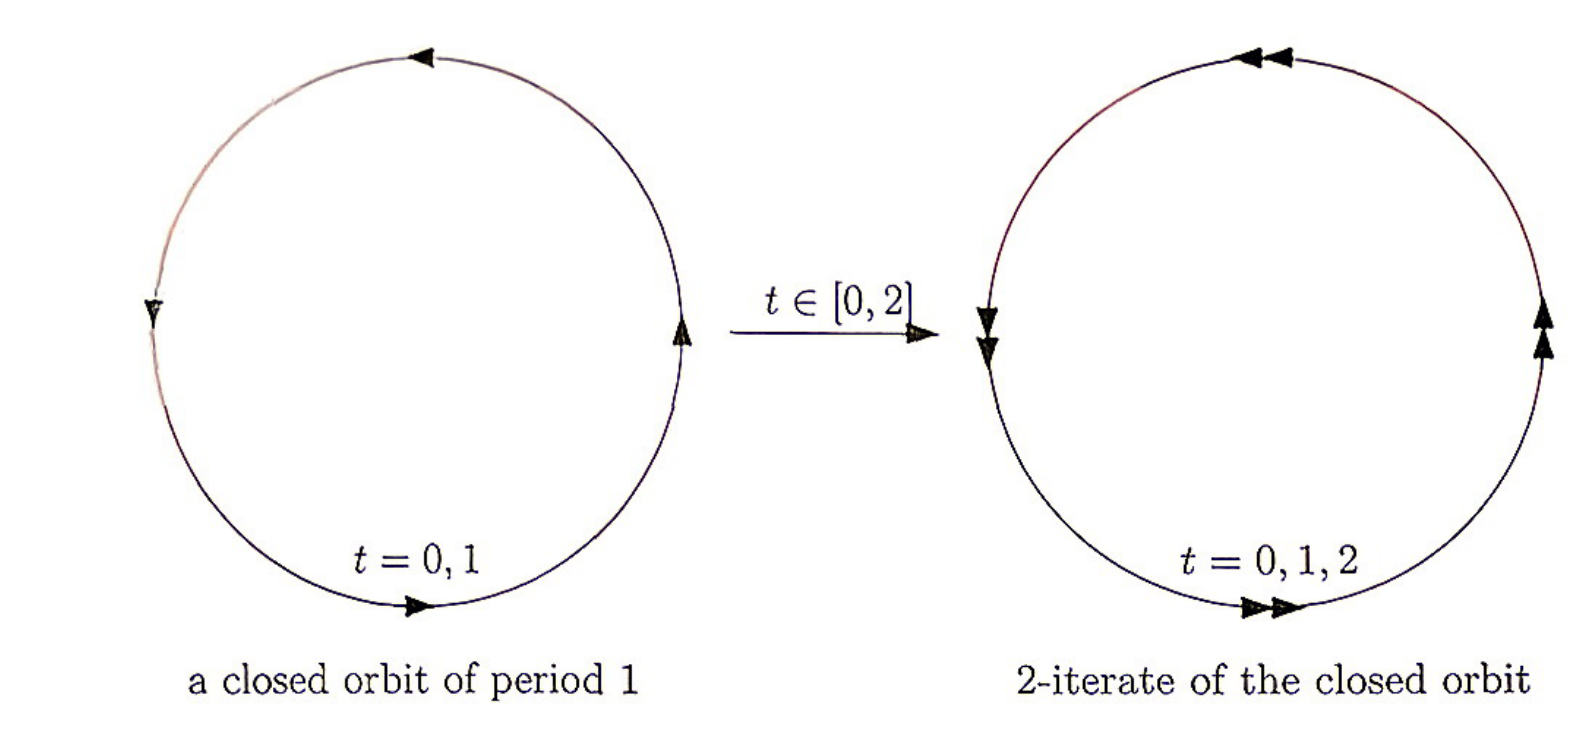
\includegraphics[width=0.72\linewidth]{figures/fig_p132_1.png}
  \caption*{图 5.15\quad 一条闭轨道及其迭代（原书 p.124, Figure 5.15）}
\end{figure}

人们可能会问：当 $t\to\infty$ 时，是否所有闭哈密顿轨道都是迭代（即属于类型 (i)）？对闭 Reeb 轨道
也可以提同样的问题。下面这个猜想断言了相反的结论。

\begin{wconj}{5.3.5}（Conley 猜想, Conley Conjecture）
  设 $(M,\omega)$ 是闭辛流形，$H\colon\R\times M\to\R$（由定义在 $[0,1]\times M$ 上的哈密顿函数
  周期延拓而得）。则哈密顿流 $\{\varphi_H^t\}_{t\in[0,\infty)}$ 存在无穷多条素闭哈密顿轨道。
  对闭切触流形上的闭 Reeb 轨道，同样的结论成立。
\end{wconj}
% [Tutor Note: 术语依据——「prime closed orbit」译「素闭轨道」，取数论中 prime 的「素的」义，
%  即不是任何轨道的非平凡迭代；不要译成「主闭轨道」（principal 的译法）。Conley 猜想预测
%  「要么只有有限条、要么无穷多条」这一二分性的「无穷」一侧，其精确表述与「通有」假设有关；
%  例 5.3.4--例 5.3.5 说明不加条件时结论会失效。]

有趣的是，猜想 5.3.5 关于闭哈密顿轨道与闭 Reeb 轨道的结论，在一般情况下都不成立。

\begin{wexam}{5.3.4}
  如图 5.13 那样，取 $(S^2,\omega_{\mathrm{area}})$ 上沿 $z$ 轴的旋转作为哈密顿微分同胚
  $\varphi$。若 $\varphi$ 是无理旋转（即沿 $z$ 轴旋转一个无理角），则对任意 $k\in\N$，$k$ 次迭代
  $\varphi^k$ 只有两个不动点。因此，由于不动点与（周期）闭哈密顿轨道之间的对应（见注 5.4.2），
  这两个不动点就是哈密顿流在 $t\to\infty$ 时仅有的闭哈密顿轨道。\hfill$//$
\end{wexam}

\begin{wexam}{5.3.5}
  在 Riemann 几何中，A. Katok 发现 $S^2$ 上一个著名的 Finsler 度量 $g$ 只承认两条素闭测地线
  [136, 247]。考虑例 3.2.4 中由 (3.12) 定义的闭切触流形——单位余球面丛
  $(S_g^*S^2,\omega_{\mathrm{can}})$。例 3.2.4 末尾导出的结论（把闭 Reeb 轨道与底流形中的闭测地线
  等同起来）对 Finsler 度量同样成立（见 [67] 第 2 节）。于是，关于 Katok 的度量，
  $(S_g^*S^2,\omega_{\mathrm{can}})$ 只承认有限多条素闭 Reeb 轨道。\hfill$//$
\end{wexam}
% >>> p133
寻找使猜想 5.3.5 成立的充分条件，是辛几何与切触几何中一个热门课题。这一方向上的近期进展见
[195, 56, 85, 144, 93]。

本节最后，我们指出例 5.3.4 与例 5.3.5 中共有的一个现象，它揭示了动力学中某种深刻的原理。
在例 5.3.4 中，若哈密顿微分同胚 $\varphi$ 不是无理旋转，即存在 $N\in\N$ 使 $N$ 次迭代
$\varphi^N=\mathbf{1}$ 在 $S^2$ 上成立，则显然会有无穷多个不动点，从而有无穷多条素闭哈密顿轨道。
因此在这一情形我们有\textbf{二分性}（dichotomy）：要么始终只有两条闭哈密顿轨道（事实上是常值轨道），
要么有无穷多条闭哈密顿轨道。在例 5.3.5 中，Bangert--Franks--Hingston 的一个著名结果
[22, 84, 116] 说：在 $S^2$ 上，要么只有两条素闭测地线（这可由 Katok 的 Finsler 度量实现），
要么有无穷多条素闭测地线。因此，提升到单位余球面丛之后，关于素闭 Reeb 轨道的基数我们也有同样的
二分性。

在辛几何中，这类二分性的结论由下述猜想给出（见 [124] 第 263 页倒数第二段）。

\begin{wconj}{5.3.6}（Hofer--Zehnder）
  设 $(M,\omega)$ 是紧辛流形，$H\colon[0,1]\times M\to\R$ 是哈密顿函数。若
  \[
    \#\mathrm{Fix}(\varphi_H^1)>\sum_i b_i(M;\mathbf{k}),
  \]
  即严格大于猜想 5.3.1 中的下界，则 $\#\mathrm{Fix}(\varphi_H^1)=\infty$。
\end{wconj}
% [Tutor Note: 易错预警——原文在此没有假定 $H$ 非退化，也没有说明 $\#$ 是否按重数
%  （局部 Floer 同调的重数）计数，而这两点在文献中恰是关键约定：只有当允许 $H$ 退化、
%  或把每个不动点按其局部 Floer 同调重数计数时，「严格大于下界必导致不动点无穷多」才与
%  Floer 理论相容。若只按普通非退化 $H$ 的不动点个数读，则 Floer 复形的生成元个数本就可以
%  大于同调群的秩 $\sum_i b_i$，字面结论会过强。核对时以 Hofer--Zehnder 原书 p.263 的原文
%  与 E. Shelukhin [204] 定理 A 的精确表述为准；本节只作性质性介绍。]

猜想 5.3.6 的一个同调版本已由 E. Shelukhin 证明（[204] 中的定理 A），其证明巧妙地综合了现代
辛几何中若干精密工具。

在切触几何中，一个受 Hofer--Wysocki--Zehnder 的开创性工作 [123] 启发的民间猜想（folklore
conjecture）如下。

\begin{wconj}{5.3.7}
  设 $(M^{2n+1},\xi)$ 是切触流形。则对 $\xi$ 的任意切触形式 $\alpha$，关于 Reeb 向量场
  $R_\alpha$ 的素闭 Reeb 轨道或者有 $\bigl\lfloor\frac{n+1}{2}\bigr\rfloor+1$ 条，或者有无穷多条。
\end{wconj}
% [Tutor Note: 易错预警——请把 $\lfloor (n+1)/2\rfloor+1$ 与维数对上号：当 $\dim M=3$（即 $n=1$）
%  时它给出 $2$，这与 Cristofaro-Gardiner--Hutchings 关于「闭 3-维切触流形上任何 Reeb 流至少有
%  两条闭轨道」的定理相符；当 $\dim M=2n+1$ 一般时它只是猜想。原文「there are either … or
%  infinitely many」是二择一的表述，不可读成「至少有 … 条且可能无穷多」。
%  另：原文写作 Hofer-Wyoscki-Zehnder，Wysocki 拼写有误，应为 Wysocki。]

这一方向已取得相当多的进展，尤其是在三维情形（见 [60, 59]），大多基于 ECH 机器。在更高维情形，
目前探索与已知都还很少。
